\appendix
\section{Specifica dei test}
\subsection{Test di validazione}
Questo tipo di test verrà utilizzato durante l'attività di collaudo del prodotto finale così da accertare che esso soddisfi le richieste del committente. \\
Per ogni test viene specificato il proprio codice univoco, la descrizione, lo stato di implementazione attuale ed il codice identificativo del requisito -o dei requisiti- ad esso associato. 

	\begin{longtable}{|>{\centering\arraybackslash}m{1.6cm}|>{\centering\arraybackslash}m{6.41cm}|>{\centering\arraybackslash}m{3.1cm} | >{\centering\arraybackslash}m{2.6cm}|}		
		\rowcolor{LightBlue}
		\textbf{\textcolor{white}{Codice}}
		& \multicolumn{1}{|c|}{\textbf{\textcolor{white}{ Descrizione}}}
		& \textbf{\textcolor{white}{Esito}} & \textbf{\textcolor{white}{Requisito associato}}\\
		TV-RO1 & L'utente non riconosciuto vuole registrarsi alla piattaforma come allievo, creando un account personale. All'utente è richiesto di:
		\begin{itemize}
			\item Raggiungere la pagina di registrazione;
			\item Inserire i dati richiesti quali:
				\begin{itemize}
				 	\item nome;
				 	\item cognome;
				 	\item username;
				 	\item email;
				 	\item password;
				 	\item nome della scuola di appartenenza;
				 	\item città sede della scuola di appartenenza;
				\end{itemize}
			\item Confermare la registrazione.
		\end{itemize} & Non implementato & ROF1, ROF24, ROF25, ROF26, ROF27, ROF28, ROF29, ROF30 \\ \hline
		\rowcolor{LightGray}
		TV-RO2 & L'utente non riconosciuto vuole registrarsi alla piattaforma come insegnante, creando un account personale. All'utente è richiesto di:
		\begin{itemize}
			\item Raggiungere la pagina di registrazione;
			\item Inserire i dati richiesti quali:
				\begin{itemize}
				 	\item nome;
				 	\item cognome;
				 	\item username;
				 	\item email;
				 	\item password;
				 	\item nome della scuola di appartenenza;
				 	\item città sede della scuola di appartenenza;
				 	\item codice INPS;
				\end{itemize}
			\item Confermare la registrazione.
		\end{itemize} & Non implementato & ROF22, ROF31, ROF24, ROF25, ROF26, ROF27, ROF28, ROF29, ROF30 \\ \hline
		TV-RO3 & L'utente non riconosciuto vuole eseguire l'accesso alla piattaforma tramite le sue credenziali. All'utente è richiesto di: 
		\begin{itemize}
			\item Raggiungere la pagina di autenticazione;
			\item Inserire il proprio username e password;
			\item Confermare l'accesso.
		\end{itemize} & Non implementato 
		& ROF2, ROF33, ROF34 \\ \hline
		  \rowcolor{LightGray}
		TV-RD1 & L'utente vuole modificare i dati del proprio profilo personale. All'utente è richiesto di:
		\begin{itemize}
			\item Raggiungere la pagina di modifica dei dati dal profilo;
			\item Modificare una o più voci tra username, password, scuola e città;
			\item Confermare la modifica.
		\end{itemize}& Non implementato  & RDF1, RDF26, RDF27, RDF28, RDF29\\ \hline
		TV-RD2 & Il  moderatore vuole verificare le credenziali di un utente che vuole registrarsi come insegnante. Al moderatore è richiesto di:
		\begin{itemize}
			\item Raggiungere la pagina di amministrazione della piattaforma;
			\item Visualizzare la lista degli utenti che richiedono i  ruolo di insegnante;
			\item Il moderatore seleziona uno degli utenti;
			\item Il moderatore accetta o rifiuta l'utente selezionato.
		\end{itemize}& Non implementato  & RDF2 \\ \hline
		  \rowcolor{LightGray}
		TV-RD3 & L'utente vuole registrarsi alla piattaforma. 
		\begin{itemize}
			\item L'utente inserisce delle credenziali errate;
			\item L'utente visualizza un messaggio di errore.
		\end{itemize}& Non implementato  & RDF3 \\ \hline
		TV-RO4 & L'utente vuole cercare degli esercizi sulla piattaforma. All'utente è richiesto di:
		\begin{itemize}
			\item Raggiungere la pagina di ricerca degli esercizi;
			\item Scrivere una frase o parte di essa nella barra di ricerca;
			\item Selezionare, eventualmente, dei filtri per la ricerca;
			\item Avviare la ricerca.
		\end{itemize}& Non implementato  & ROF3 RPF1 RPF2 RPF3 RPF4\\ \hline
		  \rowcolor{LightGray}
		TV-RD4 & L'allievo vuole visualizzare la lista delle classi a cui appartiene. All'allievo è richiesto di: 
		\begin{itemize}
			\item Accedere alla pagina dedicata al proprio profilo;
			\item Selezionare l'opzione "lista delle classi".
		\end{itemize}& Non implementato  & RDF4 \\ \hline
		TV-RP1 & Il moderatore vuole eliminare un utente iscritto alla piattaforma. Al moderatore è richiesto di: 
		\begin{itemize}
			\item Visualizzare la lista degli utenti iscritti nella piattaforma;
			\item Indicare uno o più utenti da eliminare;
			\item Confermare l'eliminazione degli utenti  selezionati.
		\end{itemize}& Non implementato  & RPF5 \\ \hline
		  \rowcolor{LightGray}
		TV-RP2 & L'insegnante vuole modificare una soluzione di un esercizio da lui fornita. All'insegnante è richiesto di: 
		\begin{itemize}
			\item Selezionare la lista degli esercizi da lui inseriti;
			\item Visualizzare la precedente soluzione;
			\item Modificare le classi grammaticali della precedente soluzione;
			\item Confermare la modifica.
		\end{itemize}& Non implementato  & RPF6 \\ \hline
		TV-RD5 & L'insegnante vuole visualizzare la lista degli esercizi da lui creati. All'insegnante è richiesto di: 
		\begin{itemize}
			\item Accedere all'area del suo profilo;
			\item Selezionare la voce "esercizi inseriti".
		\end{itemize}& Non implementato  & RDF5 \\ \hline
		  \rowcolor{LightGray}
		TV-RP3 & L'insegnante vuole eliminare una soluzione di un esercizio da lui fornita. All'insegnante è richiesto di:
		\begin{itemize}
			\item Visualizzare la lista degli esercizi da lui inseriti;
			\item Selezionare una o più soluzioni da eliminare;
			\item Confermare l'eliminazione
		\end{itemize}& Non implementato  & RPF7 \\ \hline
		TV-RO5 & L'insegnante vuole inserire un esercizio nel sistema. All'insegnante è richiesto di: 
		\begin{itemize}
			\item Raggiungere la pagina di inserimento di un nuovo esercizio;
			\item Inserire una frase;
			\item Inserire una soluzione;
			\item Specificare gli argomenti;
			\item Specificare la difficoltà;
			\item Specificare se la soluzione è pubblica o privata;
			\item Confermare l'inserimento.
		\end{itemize}& Non implementato  & ROF4 ROF6 RPF8 RPF9\\ \hline
		  \rowcolor{LightGray}
		TV-RO6 & L'utente vuole svolgere un esercizio da lui indicato. All'utente è richiesto di:
		\begin{itemize}
			\item Raggiungere la pagina per l'esecuzione degli esercizi;
			\item Inserire una frase da svolgere o selezionare un esercizio dal sistema;
			\item Compilare i campi;
			\item Confermare i dati inseriti;
			\item Visualizzare la soluzione.
		\end{itemize}& Non implementato  & ROF6 ROF7 ROF8\\ \hline
		TV-RD6 & L'allievo vuole visualizzare i dati relativi ai propri progressi. All'allievo è richiesto di:
		\begin{itemize}
			\item Accedere alla vista del proprio profilo;
			\item Visualizzare i dati relativi ai propri progressi.
		\end{itemize}& Non implementato  & RDF6 \\ \hline
		  \rowcolor{LightGray}
		TV-RD7 & Lo sviluppatore vuole visualizzare la lista delle annotazioni di una particolare frase. Allo sviluppatore è richiesto di: 
		\begin{itemize}
			\item Accedere all'area dati;
			\item Scrivere una frase o parte di essa all'interno della barra di ricerca;
			\item Selezionare eventualmente i filtri di ricerca;
			\item Confermare la ricerca.
		\end{itemize}& Non implementato  & RDF7 RDF8 RDF9 RDF10 RDF18 \\ \hline
		TV-RP4 & Lo sviluppatore vuole visualizzare i dati relativi ad una particolare annotazione. Allo sviluppatore è richiesto di:
		\begin{itemize}
			\item Visualizzare la lista delle annotazioni ricercate;
			\item Selezionare un'annotazione;
			\item Visualizzare data, utente e soluzione proposta.
		\end{itemize}& Non implementato  & RPF10 \\ \hline
		  \rowcolor{LightGray}
		TV-RP5 & Lo sviluppatore vuole visualizzare lo storico delle annotazioni. Allo sviluppatore è richiesto di:
		\begin{itemize}
			\item Visualizzare la lista delle annotazioni cercate;
			\item Selezionare la voce "vedi storico".
		\end{itemize}& Non implementato  & RPF11 \\ \hline
		TV-RP6 & Lo sviluppatore vuole ordinare la lista dei risultati ottenuti dalla ricerca. Allo sviluppatore è richiesto di: 
		\begin{itemize}
			\item Visualizzare la lista delle annotazioni ricercate;
			\item Scegliere un parametro secondo il quale ordinare i risultati;
			\item Confermare l'ordinamento scelto.
		\end{itemize}& Non implementato  & RPF12 \\ \hline
		  \rowcolor{LightGray}
		TV-RO6 & Lo sviluppatore vuole scaricare un file contenente i dati relativi agli esercizi ottenuti con la ricerca. Allo sviluppatore è richiesto di:
		\begin{itemize}
			\item Visualizzare la lista delle annotazioni ricercate;
			\item Richiedere il download dei dati;
			\item Scegliere il path per il salvataggio del file;
			\item Confermare ed eseguire il salvataggio.
		\end{itemize}& Non implementato  & ROF9 \\ \hline
		TV-RP7 & Lo sviluppatore vuole visualizzare le informazioni relative ad un dataset. Allo sviluppatore è richiesto di: 
		\begin{itemize}
			\item Visualizzare la lista delle annotazioni ricercate,
			contenente l'input della frase della fase di train del software di apprendimento automatico in base alla ricerca effettuata;
			\item Richiedere il download dei dati;
			\item Scegliere il path per il salvataggio del file;
			\item Confermare ed eseguire il salvataggio.
		\end{itemize}& Non implementato  & RPF13 \\ \hline
		  \rowcolor{LightGray}
		TV-RP8 & Lo sviluppatore vuole scaricare un modello. Allo sviluppatore è richiesto di:
		\begin{itemize}
			\item Visualizzare la lista dei modelli disponibili per l'applicazione;
			\item Selezionare un modello;
			\item Selezionare l'opzione "download";
			\item Scegliere il path per il salvataggio del file;
			\item Confermare ed eseguire il salvataggio.			
		\end{itemize}& Non implementato  & RPF14 \\ \hline
		
		TV-RP9 & Lo sviluppatore creare un modello alla piattaforma. Allo sviluppatore è richiesto di:
\begin{itemize}
 \item Selezionare la voce ”Aggiungi modello”;
 \item Inserire un file contenente il dataset;
 \item Confermare la creazione.
\end{itemize}& Non implementato  & RPF15 \\ \hline

		  \rowcolor{LightGray}
TV-RP10 & Il moderatore vuole eliminare un esercizio. Al moderatore è richiesto di:
\begin{itemize}
 \item Indicare gli esercizi da eliminare;
 \item Confermare l'eliminazione dell'esercizio.
\end{itemize}& Non implementato  & RPF16 \\ \hline

TV-RO7 & L'insegnante vuole creare una classe. All'insegnante è richiesto di:
\begin{itemize}
 \item Selezionare l'opzione "Crea classe";
 \item Assegnare un nome alla classe;
 \item Assegnare una descrizione alla classe;
 \item Confermare la creazione della classe.
\end{itemize}& Non implementato  & ROF10 \\ \hline

		  \rowcolor{LightGray}
TV-RO8 & L'insegnante vuole eliminare una classe. All'insegnante è richiesto di:
\begin{itemize}
 \item Cliccare sul pulsante di eliminazione della classe;
 \item Confermare l'eliminazione della classe.
\end{itemize}& Non implementato  & ROF11 \\ \hline

TV-RO9 & L'insegnante vuole aggiungere degli alunni ad una classe. All'insegnante è richiesto di:
\begin{itemize}
 \item Selezionare l'opzione "Aggiungi alunni";
 \item Visualizzare la lista di tutti gli alunni presenti sulla piattaforma;
 \item Scrivere l'username di un alunno, o una sua parte;
 \item Selezionare gli alunni da inserire;
 \item Confermare l'inserimento.
\end{itemize}& Non implementato  & ROF12, RPF17, RPF18 \\ \hline

		  \rowcolor{LightGray}
TV-RO10 & L'insegnante vuole assegnare degli esercizi ad una classe. All'insegnante è richiesto di:
\begin{itemize}
 \item Selezionare degli esercizi in lista da assegnare;
 \item Indicare la classe a cui assegnarli;
 \item Scrivere l'username di un alunno, o una sua parte;
 \item Confermare l'assegnazione.
\end{itemize} & Non implementato & ROF13 \\ \hline

TV-RP11 & L'insegnante vuole visualizzare i progressi di un alunno della classe. All'insegnante è richiesto di:
\begin{itemize}
 \item Selezionare uno studente;
 \item Visualizzare i grafici che riportano la media totale, la media per tipologia di
 esercizi e lo sviluppo della media nel tempo.
\end{itemize} & Non implementato & RPF19 \\ \hline
		
		  \rowcolor{LightGray}
	TV-RO11 & L'insegnante vuole eliminare un alunno dalla lista degli iscritti ad una classe. All'insegnante è richiesto di:
		\begin{itemize}
			\item Visualizzare la lista degli alunni della classe;
			\item Selezione l'allievo da rimuovere dalla classe;
			\item Confermare l'eliminazione.		
		\end{itemize} & Non implementato & ROF14 \\ \hline	
		
		TV-RO12 & L'insegnante vuole visualizzare la lista degli alunni iscritti ad una delle sue classi. All'insegnante è richiesto di:
		\begin{itemize}
			\item Accedere alla pagina di gestione delle proprie classi;
			\item Selezionare la voce "vedi alunni".		
		\end{itemize}& Non implementato  & ROF15 \\ \hline
		
		  \rowcolor{LightGray}
		TV-RO13 & L'insegnante vuole visualizzare la lista delle proprie classi. All'insegnante è richiesto di:
		\begin{itemize}
			\item Accedere alla pagina del proprio profilo;
			\item Selezionare la voce "vedi classi".		
		\end{itemize} & Non implementato & ROF16 \\ \hline
		
		TV-RD7 & L'allievo vuole annullare l'iscrizione ad una classe. Allo studente è richiesto di:
		\begin{itemize}
			\item Visualizzare la lista delle classi a cui appartiene;
			\item Selezionare l'opzione "disiscriviti".		
		\end{itemize}& Non implementato  & RDF11 \\ \hline
		
		  \rowcolor{LightGray}
		TV-RO14 & L'utente vuole autenticarsi alla piattaforma. 
		\begin{itemize}
			\item L'utente inserisce delle credenziali errate;
			\item L'utente visualizza un messaggio di errore.
		\end{itemize} & Non implementato & RDF17 \\ \hline
		
		TV-RO15 & L'utente vuole modificare le proprie credenziali. 
		\begin{itemize}
			\item L'utente inserisce delle credenziali errate;
			\item L'utente visualizza un messaggio di errore.
		\end{itemize} & Non implementato & RDF18 \\ \hline
		
		  \rowcolor{LightGray}
  TV-RP12 & L’allievo vuole selezionare un esercizio assegnato. All'allievo è richiesto di:
  \begin{itemize}
   \item Visualizzare le informazioni della classe indicata
   \item Selezionare un esercizio assegnato
  \end{itemize} & Non implementato & RPF28 \\ \hline

 TV-RO16 & L’insegnante vuole accedere all’area di inserimento nuovo esercizio. All'insegnante è richiesto di:
 \begin{itemize}
  \item Raggiungere la vista principale dell’applicazione.
  \item Selezionare la voce ”Inserisci esercizio”
 \end{itemize} & Non implementato & ROF23 \\ \hline
  \rowcolor{LightGray}
  TV-RD8 & L’utente riconosciuto vuole disconnettersi dalla piattaforma. All'utente è richiesto di:
  \begin{itemize}
   \item Selezionare l’opzione ”Logout” da qualsiasi vista dell'applicazione
  \end{itemize} & Non implementato & RDF25 \\ \hline
 
 TV-RP13 & Lo sviluppatore vuole visualizzare informazioni riguardanti i modelli disponibili nella piattaforma. Allo sviluppatore è richiesto:
 \begin{itemize}
  \item  Visualizzare la lista dei modelli disponibili per l’applicazione;
  \item Selezionare un modello
  \item Selezionare l’opzione ”Visualizza informazioni”
 \end{itemize} & Non implementato & RPF26 \\ \hline

\rowcolor{LightGray}
TV-RD9 & Lo sviluppatore vuole visualizzare la lista dei modelli disponibili.  Allo sviluppatore è richiesto di:

\begin{itemize}
 \item Raggiungere la vista dell’area dati.
 \item Selezionare la voce ”Lista dei modelli”
\end{itemize} & Non implementato & RDF23 \\ \hline

TV-RD10 & L’utente riconosciuto vuole accedere alla vista del proprio profilo personale. All'utente è richiesto di:
\begin{itemize}
  \item Raggiungere la vista principale dell'applicazione;
 \item Selezionare la voce ”Profilo personale”.
\end{itemize} & Non implementato & RDF22 \\ \hline

\rowcolor{LightGray}
TV-RD11 & L’insegnante vuole ricercare gli esercizi che ha inserito inserendo la frase o una parte di essa. All'insegnante è richiesto di:


\begin{itemize}
 \item Visualizzare la lista degli esercizi che ha inserito nella piattaforma;
 \item Scrivere nella barra di ricerca una frase o una sua parte.
\end{itemize} & Non implementato & RDF21 \\ \hline

TV-RP14 & Il moderatore vuole ricercare gli utenti inserendo l’username o una parte di esso. Al moderatore è richiesto di:
\begin{itemize}
 \item Visualizzare la lista degli utenti presenti nella piattaforma;
 \item Scrivere nella barra di ricerca una stringa.
\end{itemize} & Non implementato & RPF25 \\ \hline

		  \rowcolor{LightGray}
TV-RD12 & Il moderatore vuole visualizzare la lista degli utenti iscritti alla piattaforma. Al moderatore è richiesto di:
\begin{itemize}
 \item Raggiungere la vista di amministrazione dell’applicazione;
 \item Selezionare l’opzione ”Utenti”.
\end{itemize} & Non implementato & RDF20 \\ \hline

TV-RP15 & Il moderatore vuole ricercare gli esercizi inserendo la frase o una parte di essa. Al moderatore è richiesto di:

\begin{itemize}
 \item Raggiungere la lista degli esercizi inseriti nella piattaforma.
 \item Scrivere nella barra di ricerca una frase o una sua parte.
\end{itemize} & Non implementato & RPF24 \\ \hline

		  \rowcolor{LightGray}
TV-RD13 & Il moderatore vuole visualizzare la lista degli esercizi inseriti nella piattaforma. Al moderatore è richiesto di:

\begin{itemize}
 \item Raggiungere la vista di amministrazione dell’applicazione.
 \item Visualizzare la lista degli esercizi inseriti nella piattaforma.
\end{itemize} & Non implementato & RDF19 \\ \hline

TV-RD14 & L’insegnante vuole visualizzare l’area per la gestione delle classi. All'insegnante è richiesto di:

\begin{itemize}
 \item Raggiungere la lista delle classi create;
 \item Visualizzare la vista di gestione di una propria classe. piattaforma.
\end{itemize} & Non implementato & RDF17 \\ \hline

		  \rowcolor{LightGray}
TV-RP16 & Il moderatore vuole eliminare una segnalazione dalla relativa lista. Al moderatore è richiesto di:

\begin{itemize}
 \item Visualizzare la lista delle segnalazioni ricevute;
 \item Selezionare la segnalazione piattaforma;
 \item Selezionare l’opzione ”Elimina segnalazione”.
\end{itemize} & Non implementato & RPF23 \\ \hline
TV-RP17 & Il moderatore vuole visualizzare la lista delle segnalazioni effettuate dagli utenti. Al moderatore è richiesto di:

\begin{itemize}
 \item Raggiunge la vista di amministrazione dell’applicazione;
 \item Selezionare l’opzione ”Lista delle segnalazioni”.
\end{itemize} & Non implementato & RPF22 \\ \hline

		  \rowcolor{LightGray}
TV-RP18 & L’utente vuole segnalare un esercizio per abuso delle regole comportamentali. All'utente è richiesto di:

\begin{itemize}
 \item Raggiunge la vista di svolgimento di un esercizio che ritiene non conforme alle norme di comportamento;
 \item Selezionare l’opzione ”Segnala abuso”.
\end{itemize} & Non implementato & RPF21 \\ \hline

TV-RO17 & L’utente vuole aggiungere una frase e svolgerla come esercizio. All'utente è richiesto di:

\begin{itemize}
 \item Raggiunge la vista principale dell’applicazione;
 \item Scrivere la frase da svolgere come esercizio;
 \item Confermare la frase indicata
\end{itemize} & Non implementato & ROF20 \\ \hline

		  \rowcolor{LightGray}
TV-RD15 & L’utente vuole accedere alla pagina di registrazione alla piattaforma. All'utente è richiesto di:

\begin{itemize}
 \item Raggiunge la vista principale dell’applicazione;
 \item Selezionare l’opzione ”Registrati”.
\end{itemize} & Non implementato & RDF24 \\ \hline

TV-RO18 & L’insegnante vuole visualizzare un messaggio di errore nel caso in cui stia inserendo una frase vuota come esercizio. All'insegnante è richiesto di:

\begin{itemize}
 \item Raggiunge la vista di inserimento di un nuovo esercizio e ha inserito;
 \item Visualizza un messaggio di errore ”La frase inserita è vuota”.
\end{itemize} & Non implementato & ROF19 \\ \hline

		  \rowcolor{LightGray}
TV-RP19 & L’utente non riconosciuto vuole ricevere una e-mail per la conferma di iscrizione come insegnante. All'utente è richiesto di:

\begin{itemize}
 \item Inviare la richiesta di registrazione come insegnante;
 \item Riceve la conferma di registrazione come insegnante.
\end{itemize} & Non implementato & RPF20 \\ \hline

		\caption{Test di validazione}
\end{longtable}

\subsection{Test di sistema}
Di seguito riportiamo una tabella contenente i test di sistema che intendiamo implementare per la verifica dei requisiti funzionali specificati nell'\textit{AnalisiDeiRequisiti\_v2.0.0}. \\
Per ogni test viene specificato il proprio codice univoco, il codice identificativo del requisito ad esso associato, la descrizione e lo stato di implementazione attuale.
	\begin{longtable}{|>{\centering\arraybackslash}m{1.6cm}|>{\centering\arraybackslash}m{1.7cm}|m{6.41cm}|>{\centering\arraybackslash}m{3.1cm}|}		
		\rowcolor{LightBlue}
		\textbf{\textcolor{white}{Codice\newline test}}
		& \textbf{\textcolor{white}{Codice\newline requisito}}
		& \multicolumn{1}{|c|}{\textbf{\textcolor{white}{ Descrizione}}}
		& \textbf{\textcolor{white}{Stato}}\\
		
		\hline
		\rowcolor{LightGray}
		TS-RO1
		& ROF32
		& Verifica che l'utente riesca a registrarsi alla piattaforma come allievo creando un account personale. 
		& non implementato\\ \hline
		\rowcolor{white}
		TS-RO2
		& ROF2 
		& Verifica che l'utente possa eseguire l'accesso alla piattaforma utilizzando le sue credenziali.
		& non implementato\\ \hline
		\rowcolor{LightGray}
		TS-RD1
		& RDF1 
		& Verifica che l'utente possa modificare i dati del proprio profilo personale.
		& non implementato\\ \hline
		\rowcolor{white}
		TS-RD2
		& RDF2 
		& Verifica che l'amministratore possa verificare le credenziali di un utente che richiede la registrazione come insegnante. 
		& non implementato\\ \hline
		\rowcolor{LightGray}
		TS-RD3
		& RDF3 
		& Verifica che l'utente venga avvisato in caso di errore nell'inserimento dei dati richiesti.
		& non implementato\\ \hline
		\rowcolor{white}
		TS-RO3		
		& ROF3 
		& Verifica che l'insegnante e l'allievo possano ricercare degli esercizi sulla piattaforma.
		& non implementato\\ \hline
		\rowcolor{LightGray}
		TS-RP1		
		& RPF1 
		& Verifica che durante la ricerca, l'utente abbia la possibilità di impostare dei filtri per raffinarla. 		
		& non implementato\\ \hline
		\rowcolor{white}
		TS-RD4		
		& RDF4 
		& Verifica che dopo una ricerca, l'utente venga avvisato con un messaggio nel caso in cui il sistema non abbia trovato nessun risultato corrispondente ai criteri selezionati.
		& non implementato\\ \hline
		\rowcolor{LightGray}
		TS-RP2		
		& RPF2 
		& Verifica che l'amministratore possa eliminare un utente iscritto alla piattaforma.
		& non implementato\\ \hline
		\rowcolor{white}
		TS-RP3		
		& RPF3 
		& Verifica che l'insegnante possa modificare una soluzione di un esercizio da lui fornita
		& non implementato\\ \hline
		\rowcolor{LightGray}
		TS-RD5		
		& RDF5 
		& Verifica che l'insegnante, accedendo alla sua area del profilo, possa visualizzare la lista degli esercizi da lui creati. 
		& non implementato\\ \hline
		\rowcolor{white}
		TS-RP4		
		& RPF4 
		& Verifica che l'insegnante possa eliminare una soluzione di un esercizio da lui fornita. 
		& non implementato\\ \hline
		\rowcolor{LightGray}
		TS-RP5		
		& RPF5 
		& Verifica che l'insegnante possa indicare gli argomenti trattati nell'esercizio in fase di creazione.
		& non implementato\\ \hline
		\rowcolor{white}
		TS-RO4		
		& ROF4 
		& Verifica che l'allievo possa inserire una frase da svolgere o selezionare un esercizio da quelli disponibili sul sistema.
		& non implementato\\ \hline
		\rowcolor{LightGray}
		TS-RO5		
		& ROF5 
		& Verifica che l'allievo possa compilare i campi relativi alle parole della frase al fine di completare l'esercizio selezionato.
		& non implementato\\ \hline
		\rowcolor{white}
		TS-RD6		
		& RDF6 
		& Verifica che lo sviluppatore possa ricercare le annotazioni di una particolare frase.
		& non implementato\\ \hline
		\rowcolor{LightGray}
		TS-RP6		
		& RPF6 
		& Verifica che lo sviluppatore possa ordinare la lista dei risultati ottenuti dalla ricerca tramite determinati parametri. 
		& non implementato\\ \hline
		\rowcolor{white}
		TS-RP7		
		& RPF7 
		& Verifica che l'amministratore possa eliminare uno qualsiasi degli esercizi inseriti nel sistema.
		& non implementato\\ \hline
		\rowcolor{LightGray}
		TS-RO6		
		& ROF6 
		& Verifica che l'insegnante possa inserire un esercizio nel sistema, indicando una soluzione per esso. 
		& non implementato\\ \hline
		\rowcolor{white}
		TS-RO7		
		& ROF7 
		& Verifica che l'insegnante possa inserire la soluzione dell'esercizio che sta creando; può renderla pubblica o privata. 
		& non implementato\\ \hline
		\rowcolor{LightGray}
		TS-RO8		
		& ROF8 
		& Verifica che l'allievo possa svolgere un esercizio da lui indicato e visualizzarne la relativa valutazione. 
		& non implementato\\ \hline
		\rowcolor{white}
		TS-RD7		
		& RDF7 
		& Verifica che l'allievo, accedendo al proprio profilo, possa visualizzare dei dati relativi ai propri progressi. 
		& non implementato\\ \hline
		\rowcolor{LightGray}
		TS-RD8		
		& RDF8 
		& Verifica che lo sviluppatore possa filtrare i dati trovati durante la ricerca ottenendo una lista di esercizi. 
		& non implementato\\ \hline
		\rowcolor{white}
		TS-RD9
		& RDF9 
		& Verifica che lo sviluppatore possa impostare un filtro temporale per la ricerca degli esercizi.
		& non implementato\\ \hline
		\rowcolor{LightGray}
		TS-RD10		
		& RDF10 
		& Verifica che lo sviluppatore possa includere o escludere dalla ricerca uno o più utenti. 
		& non implementato\\ \hline 
		\rowcolor{white}
		TS-RP8		
		& RPF8 
		& Verifica che lo sviluppatore possa visualizzare i dati relativi ad una particolare annotazione. 		
		& non implementato\\ \hline
		\rowcolor{LightGray}
		TS-RP9		
		& RPF9 
		& Verifica che lo sviluppatore possa visualizzare lo storico delle annotazioni. 
		&  non implementato\\ \hline
		\rowcolor{white}
		TS-RO9
		& ROF9 
		& Verifica che lo sviluppatore deve poter scaricare un file contenente i dati relativi agli esercizi ottenuti con la ricerca.
		& non implementato\\ \hline
		\rowcolor{LightGray}
		TS-RP10		
		& RPF10 
		& Verifica che lo sviluppatore può visualizzare le informazioni relative ad uno dei modelli disponibili. 
		& non implementato\\ \hline
		\rowcolor{white}
		TS-RP11		
		& RPF11 
		& Verifica che lo sviluppatore deve poter scaricare le informazioni riguardanti un modello. 
		& non implementato\\ \hline
		\rowcolor{LightGray}
		TS-RP12		
		& RPF12 
		& Verifica che lo sviluppatore deve poter creare un modello tramite la piattaforma. 
		& non implementato\\ \hline	
		
		\rowcolor{white}
		TS-RO10	
		& ROF10 
		& Verifica che l'insegnante possa creare una nuova classe. 
		& non implementato\\ \hline
		\rowcolor{LightGray}
		TS-RO11	
		& ROF11 
		& Verifica che l'insegnante possa eliminare una classe dal sistema. 
		& non implementato\\ \hline
		\rowcolor{white}
		TS-RO12
		& ROF12 
		& Verifica che l'insegnante possa aggiungere degli alunni ad una classe. 
		& non implementato\\ \hline
		\rowcolor{LightGray}
		TS-RO13
		& ROF13 
		& Verifica che l'insegnante possa aggiungere degli esercizi a quelli assegnati ad una classe. 
		& non implementato\\ \hline
		\rowcolor{white}
		TS-RP13
		& RPF13 
		& Verifica che l'insegnante possa visualizzare i progressi degli alunni di una propria classe.
		& non implementato\\ \hline
		\rowcolor{LightGray}
		TS-RO14
		& ROF14 
		& Verifica che l'insegnante possa eliminare un alunno dalla lista di quelli iscritti ad una delle proprie classi. 
		& non implementato\\ \hline
		\rowcolor{white}
		TS-RO15	
		& ROF15 
		& Verifica che l'insegnante possa visualizzare la lista degli alunni iscritti ad una delle sue classi. 
		& non implementato\\ \hline
		\rowcolor{LightGray}
		TS-RO16
		& ROF16 
		& Verifica che l'utente possa visualizzare la lista delle proprie classi. 
		& non implementato\\ \hline
		\rowcolor{white}
		TS-RD11	
		& RDF11 
		& Verifica che l'utente possa confermare le operazioni.
		& non implementato\\ \hline
		\rowcolor{LightGray}
		TS-RO17
		& ROF22 
		& Verifica che l'utente riesca a registrarsi alla piattaforma come insegnante creando un account personale. 
		& non implementato\\ \hline
		
		\caption{Test di sistema}
\end{longtable}

\subsection{Test di integrazione}
Questa tipologia di test serve per verificare che le varie componenti del sistema interagiscono tra loro nella maniera attesa. La strategia per definire -e poi eseguire- i seguenti test, è quella di partire dalle singole componenti per poi realizzare le varie funzionalità incrementalmente durante lo sviluppo del prodotto finale. Questo potrà essere di aiuto in caso di errori, in quanto essi si presenteranno in un ambiente già testato e funzionante. \\
Per ogni test viene specificato il suo codice univoco, la descrizione e lo stato di implementazione attuale.

	\begin{longtable}{|>{\centering\arraybackslash}m{1.6cm}|>{\centering\arraybackslash}m{6.41cm}|>{\centering\arraybackslash}m{3.1cm}|}		
		\rowcolor{LightBlue}
		\textbf{\textcolor{white}{Test}}
		& \multicolumn{1}{|c|}{\textbf{\textcolor{white}{ Descrizione}}}
		& \textbf{\textcolor{white}{Esito}}\\
		\hline
		TI1
		& Test d’integrazione front-end e back-end per la corretta visualizzazione del front-end.
		& Non implementato
		\\ \hline
		\rowcolor{LightGray}
		TI2
		& Test d’integrazione front-end e back-end per l'invio dei dati al front-end.
		& Non implementato
		\\ \hline
		TI3
		& Test d’integrazione front-end e back-end per la ricezione di dati dal front-end tramite POST.
		& Non implementato
		\\ \hline
		\rowcolor{LightGray}
		TI4
		& Test d’integrazione front-end e back-end per la ricezione di dati dal front-end tramite GET.
		& Non implementato
		\\ \hline
		TI5
		& Test d’integrazione tra back-end e Hunpos per il POS-Tagging$^*$.
		& Non implementato
		\\ \hline
		\rowcolor{LightGray}
		TI6
		& Test d’integrazione tra back-end e Hunpos per il training.
		& Non implementato
		\\ \hline	
		TI7
		& Test d’integrazione tra back-end e Google Firebase Realtime Database per la lettura dalla base di dati.
		& Non implementato
		\\ \hline	
		\rowcolor{LightGray}
		TI8
		& Test d’integrazione tra back-end e Google Firebase Realtime Database per la scrittura sulla base di dati.
		& Non implementato
		\\ \hline	
		TI9
		& Test d’integrazione tra back-end e Google Firebase Realtime Database per la modifica della base di dati.
		& Non implementato
		\\ \hline	
		\rowcolor{LightGray}
		TI10
		& Test d’integrazione tra back-end e Google Firebase Realtime Database per l'eliminazione dalla base di dati.
		& Non implementato
		\\ \hline	
		\caption{Test di integrazione}
\end{longtable}


	
\newpage
\section{Resoconto attività di verifica}
\subsection{Prodotto}
\subsubsection{Documentazione}
Nella tabella seguente vengono riportati i risultati delle verifiche eseguite sui documenti. Il resoconto contiene le verifiche sia dei documenti esterni, cioè utili al committente, sia interni, utili invece al team Ottobit.\\
	\begin{longtable}{>{\centering\arraybackslash}m{5cm} >{\centering\arraybackslash}m{4cm} >{\centering\arraybackslash}m{5cm} >{\centering\arraybackslash}m{2cm}}
		\rowcolor{LightBlue}
		\textbf{\textcolor{white}{Documento}}
		& \textbf{\textcolor{white}{Indice Gulpease}}
		& \textbf{\textcolor{white}{Esito}}\\
		\textit{StudioDiFattibilità\_v1.0.0} & 60 & Accettato\\
		\hline
		\rowcolor{LightGray}
		\textit{AnalisiDeiRequisiti\_v1.0.0} & 82 & Accettato\\
		\hline
		\textit{NormeDiProgetto\_v1.0.0} & 67 & Accettato\\
		\hline
		\rowcolor{LightGray}
		\textit{PianoDiQualifica\_v1.0.0} & 72 & Accettato\\
		\hline
		\textit{PianoDiProgetto\_v1.0.0} & 64 & Accettato\\
		\hline
		\caption{Resoconto attività di verifica per la revisione dei requisiti}
	\end{longtable}
	
	\begin{longtable}{>{\centering\arraybackslash}m{5cm} >{\centering\arraybackslash}m{4cm} >{\centering\arraybackslash}m{5cm} >{\centering\arraybackslash}m{2cm}}
		\rowcolor{LightBlue}
		\textbf{\textcolor{white}{Documento}}
		& \textbf{\textcolor{white}{Indice Gulpease}}
		& \textbf{\textcolor{white}{Esito}}\\
		\textit{StudioDiFattibilità\_v1.0.0} & 60 & Accettato\\
		\hline
		\rowcolor{LightGray}
		\textit{AnalisiDeiRequisiti\_v2.0.0} & 82 & Accettato\\
		\hline
		\textit{NormeDiProgetto\_v2.0.0} & 69 & Accettato\\
		\hline
		\rowcolor{LightGray}
		\textit{PianoDiQualifica\_v2.0.0} & 72 & Accettato\\
		\hline
		\textit{PianoDiProgetto\_v2.0.0} & 64 & Accettato\\
		\hline
		\caption{Resoconto attività di verifica per la revisione di progettazione}
	\end{longtable}


\subsubsection{Software}
Le metriche per il software non vengono calcolate fino all'inizio dell'attività di codifica. Nei processi precedenti, nonostante si sia iniziato a scrivere del codice (in funzione dello sviluppo di un \textit{Proof of Concept}$^*$), questo non viene considerato nel calcolo delle metriche.

\subsection{Processi}
\subsubsection{Valori ISO/IEC 15504 - MPC1}

GRAFICO SERIE STORICA (quando lo avremo)

\paragraph{Revisione di progetto\\}
Durante il periodo di Revisione di progetto abbiamo individuato periodicamente tutti i cambiamenti apportati ai requisiti del progetto. Questo ci ha permesso di determinare la stabilità dei requisiti nel tempo grazie all'utilizzo della metrica MPC2.
Riportiamo di seguito i calcoli e le varie rilevazioni effettuate.

\begin{longtable}{>{\centering\arraybackslash}m{3cm} >{\centering\arraybackslash}m{4cm} >{\centering\arraybackslash}m{5cm} >{\centering\arraybackslash}m{2cm}}
	\rowcolor{LightBlue}
	\textbf{\textcolor{white}{Data rilevazioni}}
	& \textbf{\textcolor{white}{Requirement Stability Index (RSI)}}
	& \textbf{\textcolor{white}{Esito}}\\
	
	2019-02-15 & \[1-\frac{0+5+4}{48}=0.81\] & Accettato\\
	\hline
	2019-02-20 & \[1-\frac{5+0+3}{43}=0.81\] & Accettato\\
	\hline
	2019-02-21 & \[1-\frac{8+0+3}{48}=0.77\] & Accettato\\
	\hline
	2019-02-22 & \[1-\frac{5+2+0}{56}=0.85\] & Accettato\\
	\hline
	2019-02-25 & \[1-\frac{11+0+0}{59}=0.81\] & Accettato\\
	\hline
	2019-02-27 & \[1-\frac{10+0+0}{70}=0.88\] & Accettato\\
	\hline
	2019-03-04 & \[1-\frac{12+0+0}{80}=0.86\] & Accettato\\
	\hline
	2019-03-05 & \[1-\frac{14+0+1}{92}=0.83\] & Accettato\\
	\hline\\
	\caption{Rilevazioni indice stabilità requisiti (RSI) - Revisione di progetto}
\end{longtable}
\begin{figure}[H]
	\centering
	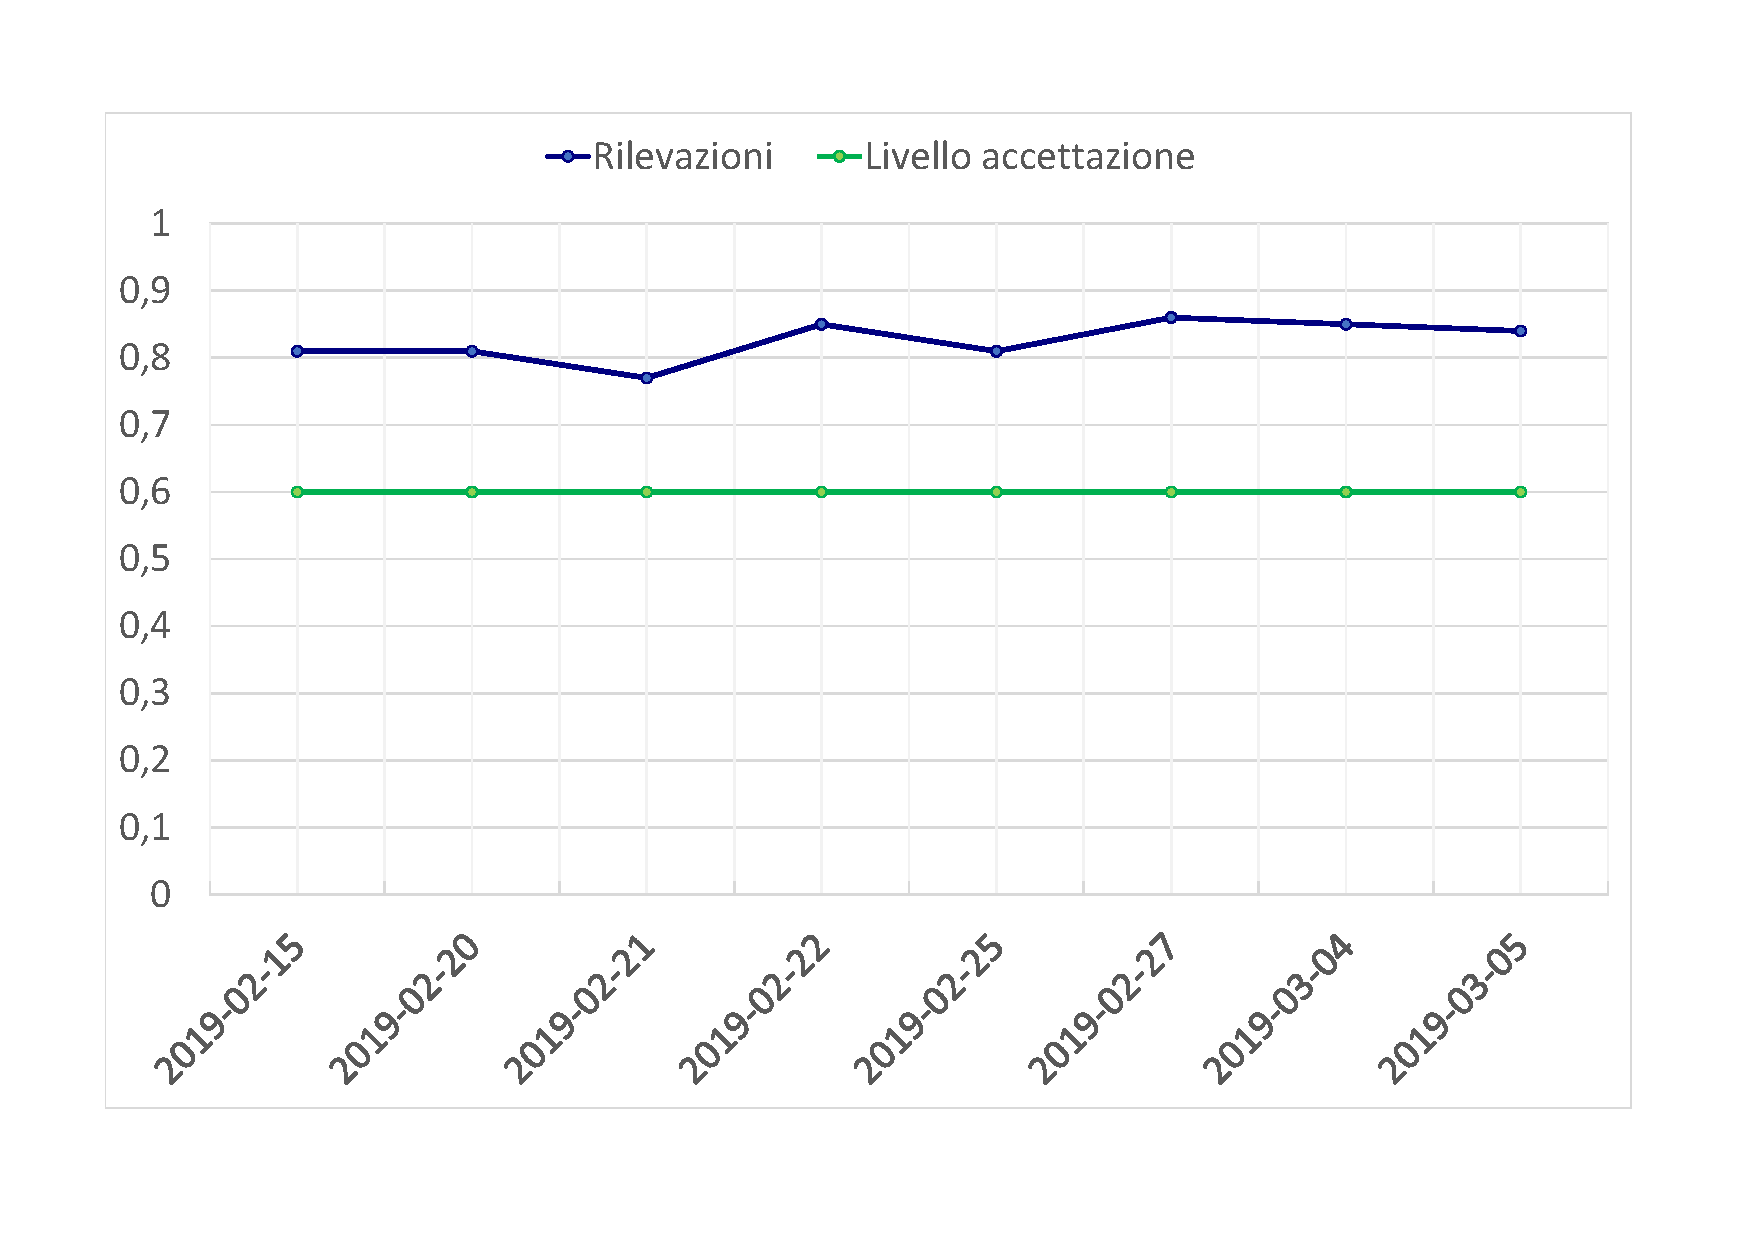
\includegraphics[scale=0.6]{images/resoconto/requisitiChart.pdf}
	\caption{Serie storica rilevazioni stabilità requisiti - Revisione di progetto}	
\end{figure}

\subsection{Esito delle revisioni - RR}
Successivamente alla prima revisione formale, il gruppo ha apportato diverse modifiche ai documenti basandosi sulle osservazioni ricevute dai docenti. Le modifiche sono riassunte di seguito:
	\begin{itemize}
		\item \textbf{Norme di Progetto}: è stata aggiunta una sezione riportante le metriche di riferimento per processi e prodotti e la relativa normazione. 
		\item \textbf{Piano di Progetto}: le attività sono state ripianificate a partire dalla fase 2 ed è stato redatto un nuovo consuntivo.
		\item \textbf{Piano di Qualifica}: la struttura del documento è stata completamente rivista, i contenuti sono stati modificati secondo le indicazioni riportate nell'esito della prima revisione. Sono stati aggiunti diversi tipi di test e diverse appendici con argomenti vari; sono stati stabiliti degli obiettivi di qualità.
		\item \textbf{Analisi dei Requisiti}: sono stati aggiunti diversi nuovi casi d'uso, specializzando quelli già presenti e raddoppiandone il numero; sono stati modificati i diagrammi UML. \`E stata aggiunta una sezione introduttiva ed una descrizione degli attori implicati nel progetto. 
	\end{itemize}

\subsection{Esito delle revisioni - RP}	

\newpage
\section{Copertura dei requisiti}
Viene riportata in seguito una tabella riassuntiva dei requisiti che non è da considerarsi definitiva, verrà infatti aggiornata in seguito ad ogni avanzamento significativo. \\
I requisiti sono indicati con il loro codice identificativo definito nel documento \textit{NormeDiProgetto\_v2.0.0} e la loro descrizione dettagliata è riportata nel documento \textit{AnalisiDeiRequisiti\_v2.0.0}.
\begin{longtable}{| p{2.5cm} | p{3cm} |}
	\rowcolor{LightBlue}
	\color{white}\bfseries Requisito & \color{white}\bfseries Stato \\
	ROF1 & Non soddisfatto \\ \hline
	ROF2 & Non soddisfatto \\ \hline
	ROF3 & Non soddisfatto \\ \hline
	ROF4 & Non soddisfatto \\ \hline
	ROF5 & Non soddisfatto \\ \hline
	ROF6 & Non soddisfatto \\ \hline
	ROF7 & Non soddisfatto \\ \hline
	ROF8 & Non soddisfatto \\ \hline
	ROF9 & Non soddisfatto \\ \hline
	ROF10 & Non soddisfatto \\ \hline
	ROF11 & Non soddisfatto \\ \hline
	ROF12 & Non soddisfatto \\ \hline
	ROF13 & Non soddisfatto \\ \hline
	ROF14 & Non soddisfatto \\ \hline
	ROF15 & Non soddisfatto \\ \hline
	ROF16 & Non soddisfatto \\ \hline
	ROF17 & Non soddisfatto \\ \hline
	ROF18 & Non soddisfatto \\ \hline
	ROF19 & Non soddisfatto \\ \hline
	ROF20 & Non soddisfatto \\ \hline
	ROF21 & Non soddisfatto \\ \hline
	ROF22 & Non soddisfatto \\ \hline
	ROF23 & Non soddisfatto \\ \hline
	ROF24 & Non soddisfatto \\ \hline
	ROF25 & Non soddisfatto \\ \hline
	ROF26 & Non soddisfatto \\ \hline
	ROF27 & Non soddisfatto \\ \hline
	ROF28 & Non soddisfatto \\ \hline
	ROF29 & Non soddisfatto \\ \hline
	ROF30 & Non soddisfatto \\ \hline
	ROF31 & Non soddisfatto \\ \hline
	ROF32 & Non soddisfatto \\ \hline
	ROF33 & Non soddisfatto \\ \hline
	ROF34 & Non soddisfatto \\ \hline
	RDF1 & Non soddisfatto \\ \hline
	RDF2 & Non soddisfatto \\ \hline
	RDF3 & Non soddisfatto \\ \hline
	RDF4 & Non soddisfatto \\ \hline
	RDF5 & Non soddisfatto \\ \hline
	RDF6 & Non soddisfatto \\ \hline
	RDF7 & Non soddisfatto \\ \hline
	RDF8 & Non soddisfatto \\ \hline
	RDF9 & Non soddisfatto \\ \hline
	RDF10 & Non soddisfatto \\ \hline
	RDF11 & Non soddisfatto \\ \hline
	RDF12 & Non soddisfatto \\ \hline
	RDF13 & Non soddisfatto \\ \hline
	RDF14 & Non soddisfatto \\ \hline
	RDF15 & Non soddisfatto \\ \hline
	RDF16 & Non soddisfatto \\ \hline
	RDF17 & Non soddisfatto \\ \hline
	RDF18 & Non soddisfatto \\ \hline
	RDF19 & Non soddisfatto \\ \hline
	RDF20 & Non soddisfatto \\ \hline
	RDF21 & Non soddisfatto \\ \hline
	RDF22 & Non soddisfatto \\ \hline
	RDF23 & Non soddisfatto \\ \hline
	RDF24 & Non soddisfatto \\ \hline
	RDF25 & Non soddisfatto \\ \hline
	RDF26 & Non soddisfatto \\ \hline
	RDF27 & Non soddisfatto \\ \hline
	RDF28 & Non soddisfatto \\ \hline
	RDF29 & Non soddisfatto \\ \hline
	RPF1 & Non soddisfatto \\ \hline
	RPF2 & Non soddisfatto \\ \hline
	RPF3 & Non soddisfatto \\ \hline
	RPF4 & Non soddisfatto \\ \hline
	RPF5 & Non soddisfatto \\ \hline
	RPF6 & Non soddisfatto \\ \hline
	RPF7 & Non soddisfatto \\ \hline
	RPF8 & Non soddisfatto \\ \hline
	RPF9 & Non soddisfatto \\ \hline
	RPF10 & Non soddisfatto \\ \hline
	RPF11 & Non soddisfatto \\ \hline
	RPF12 & Non soddisfatto \\ \hline
	RPF13 & Non soddisfatto \\ \hline
	RPF14 & Non soddisfatto \\ \hline
	RPF15 & Non soddisfatto \\ \hline
	RPF16 & Non soddisfatto \\ \hline
	RPF17 & Non soddisfatto \\ \hline
	RPF18 & Non soddisfatto \\ \hline
	RPF19 & Non soddisfatto \\ \hline
	RPF20 & Non soddisfatto \\ \hline
	RPF21 & Non soddisfatto \\ \hline
	RPF22 & Non soddisfatto \\ \hline
	RPF23 & Non soddisfatto \\ \hline
	RPF24 & Non soddisfatto \\ \hline
	RPF25 & Non soddisfatto \\ \hline
	RPF26 & Non soddisfatto \\ \hline
	RPF27 & Non soddisfatto \\ \hline
	RPF28 & Non soddisfatto \\ \hline
	ROV1 & Non soddisfatto \\ \hline
	ROV2 & Non soddisfatto \\ \hline
	ROV3 & Non soddisfatto \\ \hline
	ROV4 & Non soddisfatto \\ \hline
	ROV5 & Non soddisfatto \\ \hline
	RDV1 & Non soddisfatto \\ \hline
	RPV1 & Non soddisfatto \\ \hline
	ROQ1 & Non soddisfatto \\ \hline
	ROQ2 & Non soddisfatto \\ \hline
	ROQ3 & Non soddisfatto \\ \hline
	RDQ1 & Non soddisfatto \\ \hline
	RDQ2 & Non soddisfatto \\ \hline
	RDQ3 & Non soddisfatto \\ \hline
	RDQ4 & Non soddisfatto \\ \hline
	RDQ5 & Non soddisfatto \\ \hline
	RPQ1 & Non soddisfatto \\ \hline
	\caption{Riassunto copertura requisiti}
\end{longtable}


	
